\documentclass{article}\usepackage[]{graphicx}\usepackage[]{color}
% maxwidth is the original width if it is less than linewidth
% otherwise use linewidth (to make sure the graphics do not exceed the margin)
\makeatletter
\def\maxwidth{ %
  \ifdim\Gin@nat@width>\linewidth
    \linewidth
  \else
    \Gin@nat@width
  \fi
}
\makeatother

\definecolor{fgcolor}{rgb}{0.345, 0.345, 0.345}
\newcommand{\hlnum}[1]{\textcolor[rgb]{0.686,0.059,0.569}{#1}}%
\newcommand{\hlstr}[1]{\textcolor[rgb]{0.192,0.494,0.8}{#1}}%
\newcommand{\hlcom}[1]{\textcolor[rgb]{0.678,0.584,0.686}{\textit{#1}}}%
\newcommand{\hlopt}[1]{\textcolor[rgb]{0,0,0}{#1}}%
\newcommand{\hlstd}[1]{\textcolor[rgb]{0.345,0.345,0.345}{#1}}%
\newcommand{\hlkwa}[1]{\textcolor[rgb]{0.161,0.373,0.58}{\textbf{#1}}}%
\newcommand{\hlkwb}[1]{\textcolor[rgb]{0.69,0.353,0.396}{#1}}%
\newcommand{\hlkwc}[1]{\textcolor[rgb]{0.333,0.667,0.333}{#1}}%
\newcommand{\hlkwd}[1]{\textcolor[rgb]{0.737,0.353,0.396}{\textbf{#1}}}%
\let\hlipl\hlkwb

\usepackage{framed}
\makeatletter
\newenvironment{kframe}{%
 \def\at@end@of@kframe{}%
 \ifinner\ifhmode%
  \def\at@end@of@kframe{\end{minipage}}%
  \begin{minipage}{\columnwidth}%
 \fi\fi%
 \def\FrameCommand##1{\hskip\@totalleftmargin \hskip-\fboxsep
 \colorbox{shadecolor}{##1}\hskip-\fboxsep
     % There is no \\@totalrightmargin, so:
     \hskip-\linewidth \hskip-\@totalleftmargin \hskip\columnwidth}%
 \MakeFramed {\advance\hsize-\width
   \@totalleftmargin\z@ \linewidth\hsize
   \@setminipage}}%
 {\par\unskip\endMakeFramed%
 \at@end@of@kframe}
\makeatother

\definecolor{shadecolor}{rgb}{.97, .97, .97}
\definecolor{messagecolor}{rgb}{0, 0, 0}
\definecolor{warningcolor}{rgb}{1, 0, 1}
\definecolor{errorcolor}{rgb}{1, 0, 0}
\newenvironment{knitrout}{}{} % an empty environment to be redefined in TeX

\usepackage{alltt}

\usepackage{hyperref}

\title{Creating a Blog Template and Making Files Available for Feedback}
\IfFileExists{upquote.sty}{\usepackage{upquote}}{}
\begin{document}
\maketitle

%\section{Creating a Blog from an Rstudio Template}

%\subsection{Using the Rstudio Template} 

\section{Linking your Blog to Course \texttt{Index.html}}

\subsection{Creating a ``Hook''}

For each blog, we'll need a introductory link -- text that encourages a reader to look at your blog from the introduction that I have outline. Create a file ('File/New/Text File') and save it as 

\noindent were X is your surname. You can revise the text as you go, but include the hook in your first submission. I'll use this text to create a link to the blog. 

\subsection{Writing a ``Hook''}

In the text file, write text that can be used to link to your text. Try to write one or two sentances, at most, that describes the take home message of your blog. This should entice readers to your blog if they hit our \href{https://marclos.github.io/Climate_Change_Narratives/index.html}{landing page (index.html)}.


%called `hook' and put some text in there that can be used in the introduction and I'll create a link to your blog. 

When submiting to the Sakai site, please include the `hook' in the exported files.  

\section{Naming your Blog}

Please name your blog with your surname only, e.g. `LosHuertos.Rmd', then I can make links from the introduction you have written to your blog in a relatively straighforward way. With each new version, please add a version number, e.g. `LosHuertos2.Rmd', which will create a new html that I can link to easily by just adding the number and I don't get lost in which is most up to date. 

%\subsection{Creating a Universal Path}

%When we created our links to the files, such as our csv files, we had a long path name that links to our home directory. However, for this blogs to be posted, it's better to remove the path and just have the file name. 

%Delete all references to the path (folder structure) before the csv file name. Re-knit to make sure nothing has broken. 

\section{Cleaning up Directory}

\subsection{Creating Path to Data and Graphics Folder}

As you get ready to publish the blog, please ensure you data is moved to the 'Data/FA20' folder (Figure~\ref{fig:move}). After you move the data, change the file path in your blog and make sure it still knits. 

\begin{figure}
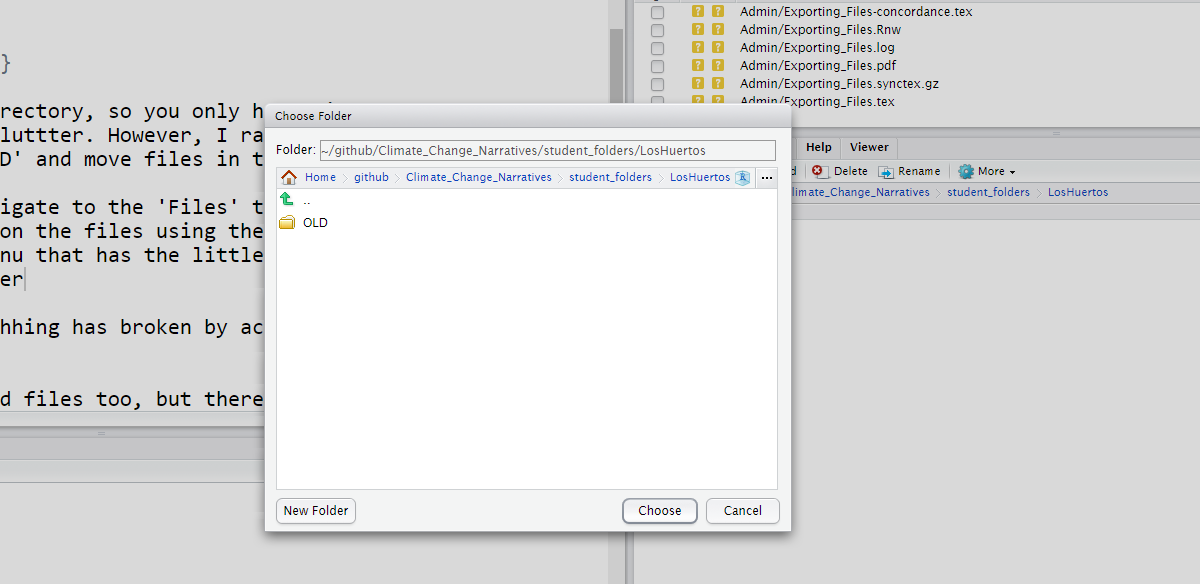
\includegraphics[width=\textwidth]{MoveFiles}
\caption{Again, moving folders is pretty straightforward, if you can select then navigate to the gear icon.}
\label{fig:move}
\end{figure}

In addition, if you have any images, create a graphics folder and put them in there. Be sure to change the link to the file in your Rmd file.

\begin{figure}
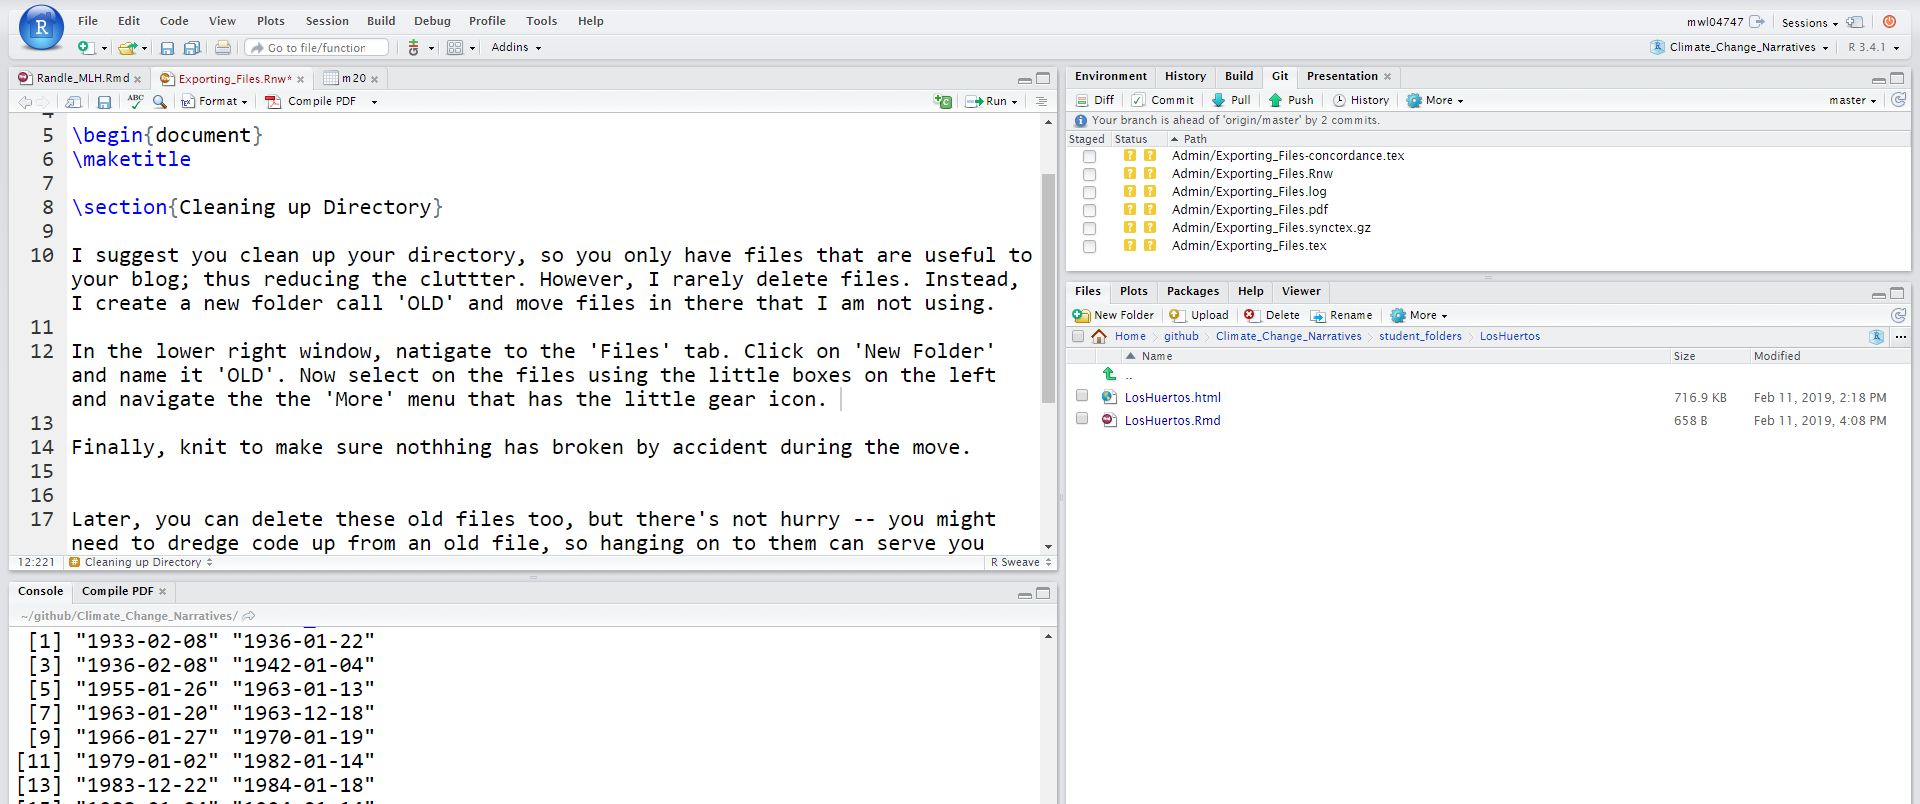
\includegraphics[width=\textwidth]{FourWindows}
\caption{Start by selecting the `Files' tab in the lower, right pane.}
\end{figure}

I suggest you clean up your directory, so you only have files that are useful to your blog; thus reducing the cluttter. However, I rarely delete files. Instead, I create a new folder call `OLD' and move files in there that I am not using.

\begin{figure}
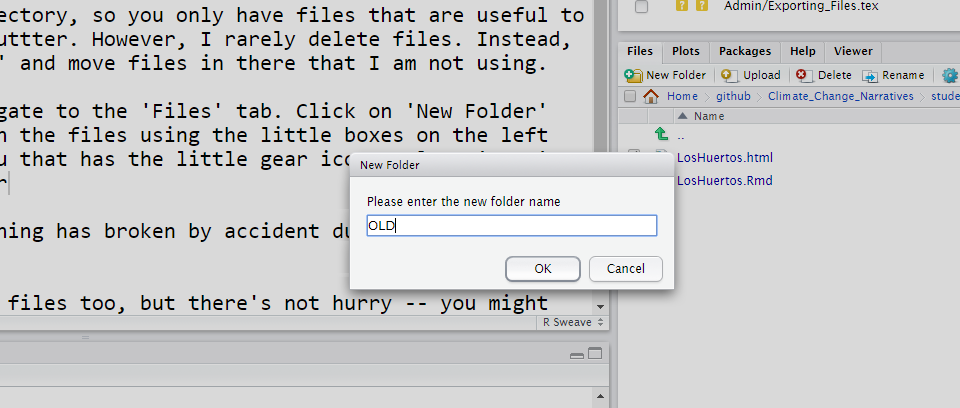
\includegraphics[width=\textwidth]{CreateFolder}
\caption{Creating the folder is easy, but relies on using the little gear icon in the files pane.}
\end{figure}

In the lower right window, natigate to the `Files' tab. Click on `New Folder' and name it `OLD'. Now select on the files using the little boxes on the left and navigate the the 'More' menu that has the little gear icon. Select `Move' and choose the `OLD' to move the files (Figure~\ref{fig:move}). Finally, knit to make sure nothhing has broken by accident during the move. 

Later, you can delete these old files too, but there's no hurry -- you might need to dredge code up from an old file, so hanging on to them can serve you later. 

\section{Exporting Files}

Similar to the moving process, you will select the files you want to export by checking the boxes on the left of the files and then navigate to the `More' menu item with the gear icon. Then select export and R studio will prompt you to determine the location you want to download the file (Figure~\ref{fig:export}).

\begin{figure}[h]
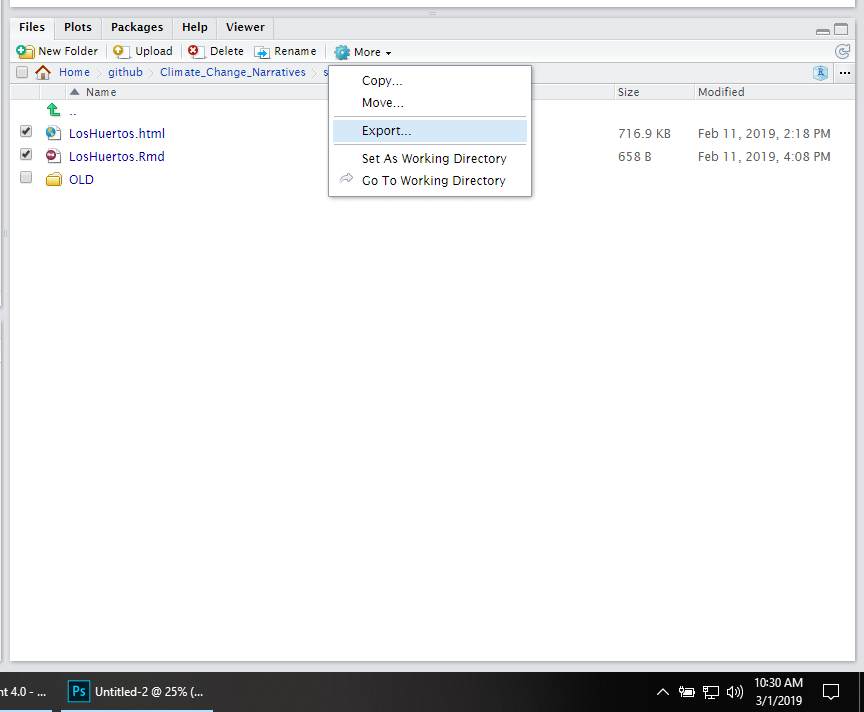
\includegraphics[width=\textwidth]{ExportFiles}
\caption{The export command creates a zip file that can downloaded to your local computer. Beware: Apple computers automatically unzip the files, which can't be uploaded to Rstudio. So, MAC users have to compress the files before uploading to Sakai.}
\label{fig:export}
\end{figure}

Note: For PC users this is a zip file that can be uploaded directly to Sakai. However, for MAC users, you must compress the file so that it can be put into Sakai. 

\subsection{Making Blogs Public}

I will copy your html files (and cleaned-up directory) into the `docs' folder, where I will knit the files to create the html. These files will by synced and publicly visible in about 10-15 minutes after I upload them. 

\end{document}
